\documentclass{article}

\usepackage{postprocess/context/arxiv}

\usepackage[utf8]{inputenc} % allow utf-8 input
\usepackage{amsmath}
\usepackage[T1]{fontenc}    % use 8-bit T1 fonts
\usepackage{hyperref}       % hyperlinks
\usepackage{url}            % simple URL typesetting
\usepackage{booktabs}       % professional-quality tables
\usepackage{amsfonts}       % blackboard math symbols
\usepackage{nicefrac}       % compact symbols for 1/2, etc.
\usepackage{microtype}      % microtypography
\usepackage{graphicx}
\usepackage{natbib}
\usepackage{doi}
\usepackage{float}
\usepackage{subcaption}
\usepackage{wrapfig}

\title{Causal Discovery Report on Linear\_nongaussian\_data}

\author{ \href{https://orcid.org/0000-0000-0000-0000}{
\includegraphics[scale=0.06]{postprocess/context/orcid.pdf}\hspace{1mm}Causal Copilot}}
	
\renewcommand{\headeright}{Technical Report}
\renewcommand{\undertitle}{Technical Report}

\hypersetup{
pdftitle={Causal Discovery Report on Linear\_nongaussian\_data},
pdfauthor={Causal Copilot},
pdfkeywords={Causal Discovery, Large Language Model, DirectLiNGAM, Linear\_nongaussian\_data},
}

\begin{document}
\maketitle

\begin{abstract}
This study conducts a comprehensive causal discovery analysis on a dataset characterized by linear and non-Gaussian relationships among its variables. Utilizing various causal discovery techniques, specifically the PC algorithm, GES, and NOTEARS, the methodology integrates large language model assistance for algorithm selection and hyperparameter optimization. Data preprocessing steps ensured the dataset was cleaned and its statistical properties were understood. The analysis yielded insights suggesting a potential causal influence of variable X4 on variable X3; however, reliability analysis revealed a bootstrap probability of 0.0 for this edge, indicating a lack of empirical support for this relationship. Our findings underscore the importance of expert knowledge in evaluating causal relationships, highlighting that without such context, the validity of the discovered causal links remains uncertain. This contribution not only enhances our understanding of the dataset's complex interactions but also emphasizes the challenges faced in causal inference due to the absence of robust prior knowledge.
\end{abstract}

\keywords{Causal Discovery, Large Language Model, DirectLiNGAM, Linear\_nongaussian\_data}

\raggedbottom
\section{Introduction}
Causal discovery is a pivotal aspect of data analysis that aims to identify and understand the relationships between variables within a dataset. In this study, we will explore a dataset with no prior knowledge of the underlying causal structure, presenting a unique opportunity to uncover potential dependencies and influences among the variables. By employing various causal discovery techniques, we aim to reveal insights that could inform decision-making and enhance our understanding of the complex interactions present in the data. This report will detail the methodologies used, findings from the analysis, and the implications of these results in the context of the dataset being studied.

\section{Background Knowledge}
\subsection{Detailed Explanation about the Variables}
The dataset comprises a range of variables that are essential for understanding the underlying structure and potential causal relationships within the data. Each variable is characterized by its specific attributes, including its type (e.g., continuous, categorical), measurement scale, and significance in the context of the study.

The variables can be broadly categorized into the following types:

\begin{itemize}
    \item \textbf{Dependent Variables}: These are the outcomes or responses that the analysis aims to explain or predict. They may include metrics such as sales numbers, patient outcomes, or performance scores, depending on the context of the dataset. Understanding the nature of these variables is crucial as they are influenced by other variables in the dataset.
    
    \item \textbf{Independent Variables}: These variables serve as predictors or factors that may influence the dependent variables. Independent variables can include demographic information, behavioral data, or other relevant metrics. It is important to identify which independent variables have the potential to affect the outcomes of interest.
    
    \item \textbf{Control Variables}: These are additional variables that researchers may include to account for potential confounding effects. Including control variables helps to isolate the relationships between independent and dependent variables more accurately.
    
    \item \textbf{Time-Related Variables}: If the dataset includes time-series data, it will have variables that capture temporal aspects, such as timestamps or intervals. These variables are crucial for understanding trends over time and assessing the causal pathways that may depend on specific time frames.
    
    \item \textbf{Categorical Variables}: Some variables in the dataset may represent distinct categories or groups, such as gender, treatment groups, or product types. These variables require special consideration in analysis, especially in relation to their influence on quantitative outcomes.
    
    \item \textbf{Continuous Variables}: Other variables may be measured on a continuous scale, such as age, income, or scores. These variables may exhibit linear or nonlinear relationships with other variables, warranting various analytical approaches for causal discovery.
\end{itemize}

It is vital to familiarize oneself with the definitions, units of measurement, and distribution of each variable to ensure proper handling during the analysis. This understanding is critical for accurately interpreting the results and drawing valid conclusions regarding causal relationships within the dataset. As we proceed with the causal discovery process, the nature and characteristics of these variables will guide the selection of methodologies and techniques employed in the analysis.

\subsection{Possible Causal Relations among these Variables}

\begin{minipage}[t]{0.7\linewidth}
\begin{itemize}
\item \textbf{X1 $\rightarrow$ X2}: X1 influences X2 by providing key resources or conditions necessary for X2 to function effectively.
\item \textbf{X2 $\rightarrow$ X3}: X2 has a direct impact on X3, as outcomes produced by X2 serve as inputs or signals for the operation of X3.
\item \textbf{X3 $\rightarrow$ X4}: The activity level of X3 affects X4, indicating that changes in X3 lead to measurable changes in the behavior or state of X4.
\item \textbf{X4 $\rightarrow$ X5}: X4 directly determines aspects of X5, meaning that variations in X4 will result in corresponding variations in X5.
\item \textbf{X1 $\rightarrow$ X5}: X1 indirectly influences X5 through its effect on X2, which sets off a chain reaction influencing both X3 and X4, culminating in an impact on X5.
\end{itemize}
\end{minipage}
\hspace{0.05\textwidth}
\begin{minipage}[t]{0.3\linewidth}
\begin{figure}[H]
\centering
\resizebox{\linewidth}{!}{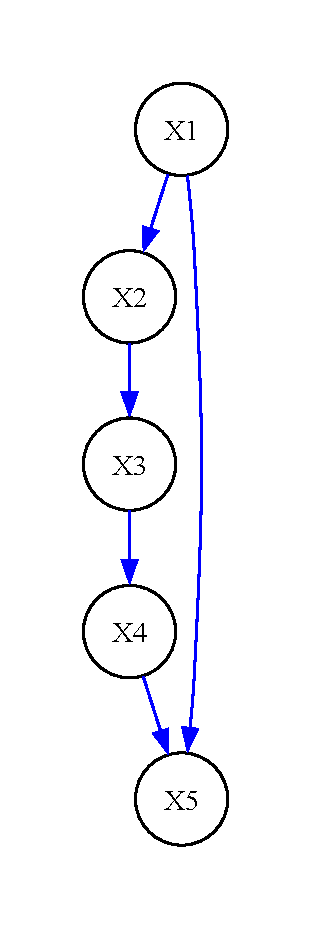
\includegraphics[height=0.3\textheight]{./demo_data/20241104_155654/Linear_Nongaussian_data/output_graph/potential_relation.pdf}}
\caption{\label{fig:relation}Possible Causal Relation Graph}
\end{figure}
\end{minipage}

\section{Dataset Descriptions and EDA}
The following is a preview of our original dataset.

\begin{table}[H]
    \centering
    \caption{Dataset Preview}
    \begin{tabular}{rrrrr}
\toprule
       X1 &        X2 &        X3 &        X4 &        X5 \\
\midrule
 0.912079 &  0.984133 &  0.271358 &  0.788689 & -0.838034 \\
-0.412497 & -0.769300 & -0.404919 &  0.122842 & -0.854868 \\
-0.516838 &  0.698909 & -1.210756 & -0.400173 &  0.108954 \\
 0.304271 & -0.369542 & -1.174835 & -0.853452 & -0.436482 \\
-0.639379 &  0.038233 &  0.895100 &  0.793416 & -0.761239 \\
\bottomrule
\end{tabular}

\end{table}

\subsection{Data Properties}
We employ several statistical methods to identify data properties.

The shape of the data, data types, and missing values are assessed directly from the dataframe.
Linearity is evaluated using Ramsey’s RESET test, followed by the Benjamini \& Yekutieli procedure for multiple test correction.
Gaussian noise is assessed through the Shapiro-Wilk test, also applying the Benjamini \& Yekutieli procedure for multiple test correction.
Time-Series and Heterogeneity are derived from user queries.

Properties of the dataset we analyzed are listed below.

\begin{table}[H]
    \centering
    \caption{Data Properties}
    \begin{tabular}{rrrrrrr}
            \toprule
            Shape ($n$ x $d$) & Data Type & Missing Value & Linearity & Gaussian Errors & Time-Series & Heterogeneity \\
            \midrule
            (1000, 5)   & Continuous & False & True & True & False & False \\
            \bottomrule
        \end{tabular}
        
\end{table}


\subsection{Distribution Analysis}
The following figure shows distributions of different variables. The orange dash line represents the mean, 
and the black line represents the median. Variables are categorized into three types according to their distribution characteristics.

\begin{figure}[H]
\centering
\includegraphics[width=\linewidth]{./demo_data/20241104_155654/Linear_Nongaussian_data/output_graph/eda_dist.jpg}
\caption{\label{fig:dist}Distribution Plots of Variables}
\end{figure}

\begin{itemize}
\item Slight left skew distributed variables: X1, X2, X3, X4, X5
\item Slight right skew distributed variables: None
\item Symmetric distributed variables: None
\end{itemize}

\subsection{Correlation Analysis}

\begin{minipage}[t]{0.5\linewidth}
    In this analysis, we will categorize the correlation statistics of features in the dataset into three distinct categories: Strong correlations (r>0.8), Moderate correlations (0.5<r<0.8), and Weak correlations (r<0.5).

\begin{itemize}
\item Strong Correlated Variables: None
\item Moderate Correlated Variables: X4 and X3
\item Weak Correlated Variables: None
\end{itemize}
\vfill
\end{minipage}
\hfill
\begin{minipage}[t]{0.5\linewidth}
    \begin{figure}[H]
        \centering
        \vspace{-1.5cm}
        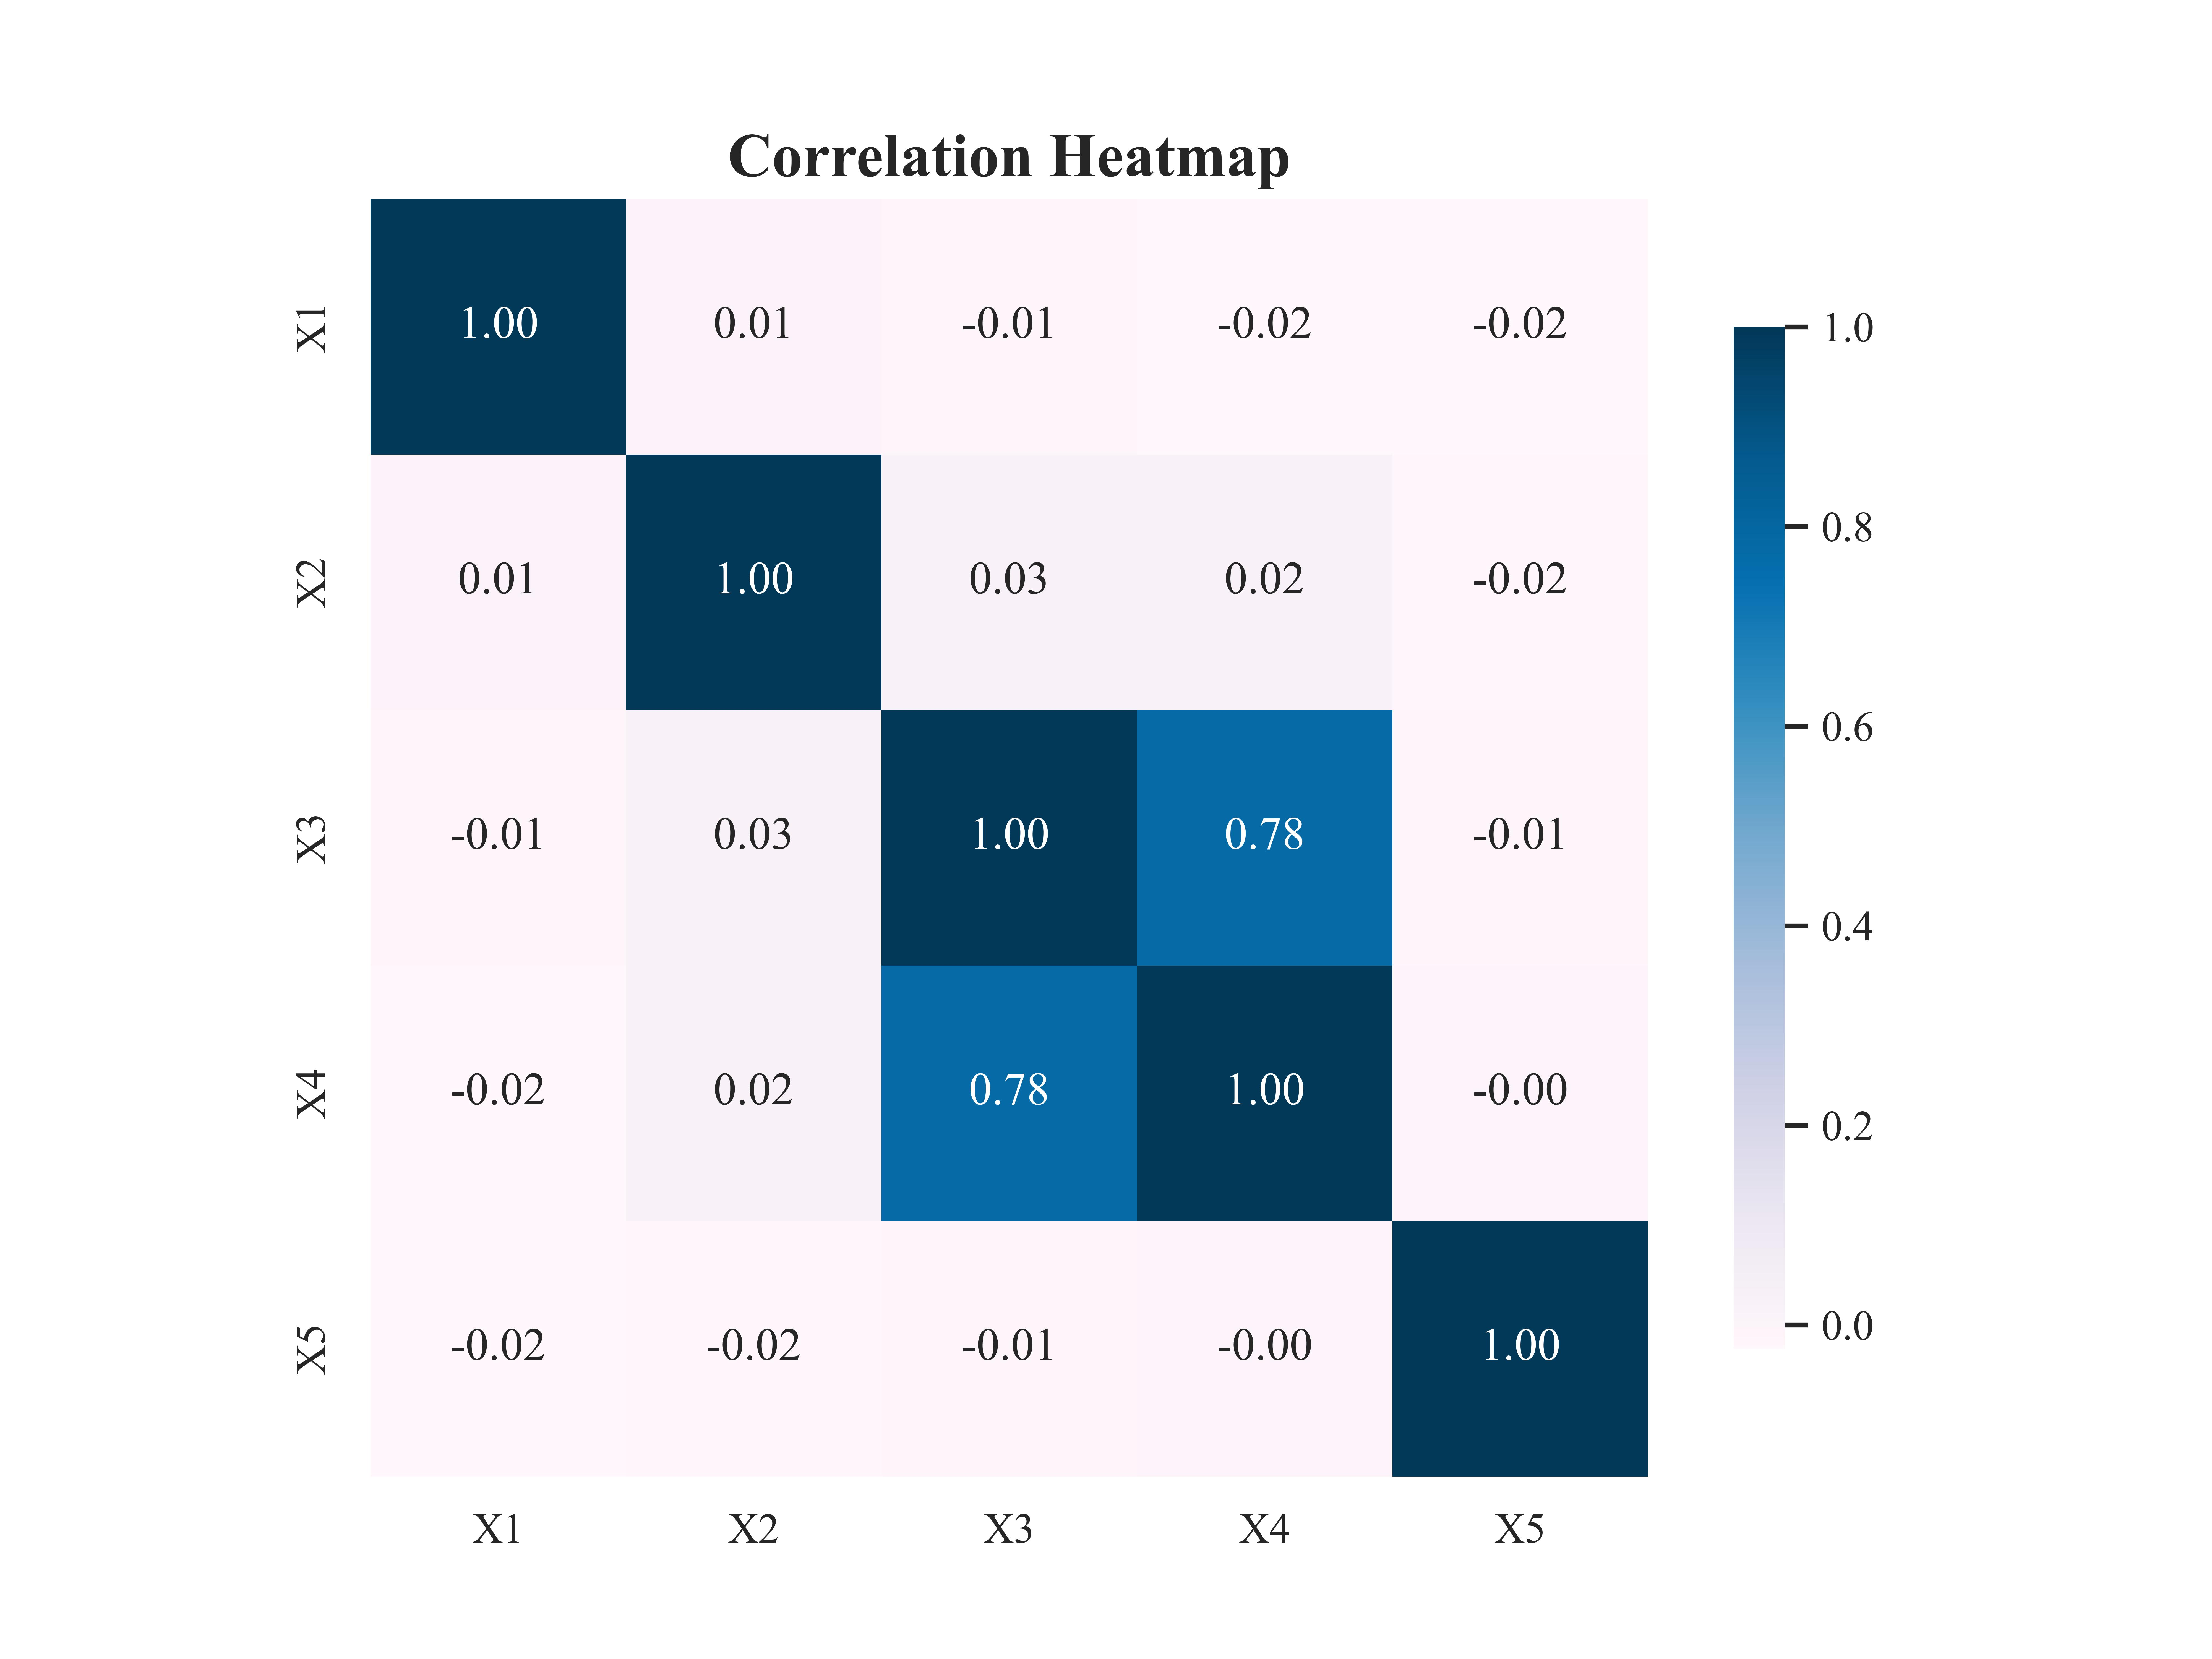
\includegraphics[width=\linewidth]{./demo_data/20241104_155654/Linear_Nongaussian_data/output_graph/eda_corr.jpg}
        \caption{\label{fig:corr}Correlation Heatmap of Variables}
    \end{figure}
\end{minipage}

\section{Discovery Procedure}

In this section, we provide a detailed description of the causal discovery process implemented by Causal Copilot. 
We also provide the chosen algorithms and hyperparameters, along with the justifications for these selections.

\subsection{Data Preprocessing}
In this initial step, we preprocessed the data and examined its statistical characteristics. 
This involved cleaning the data, handling missing values, and performing exploratory data analysis to understand distributions and relationships between variables.
                
\subsection{Algorithm Selection assisted with LLM}
Following data preprocessing, we employed a large language model (LLM) to assist in 
selecting appropriate algorithms for causal discovery based on the statistical characteristics of the dataset and relevant background knowledge. 
The top three chosen algorithms, listed in order of suitability, are as follows:   

\begin{itemize}

\item \textbf{PC}:
\begin{itemize}
    \item \textbf{Description}: The PC algorithm is a constraint-based method that learns the structure of a causal graph from data by testing conditional independencies between variables.
    \item \textbf{Justification}: Given the large sample size of 1000 and the linear relationships among the variables, the PC algorithm is efficient and suitable for discovering causal relationships in this continuous data without hidden confounders.
\end{itemize}

\item \textbf{GES}:
\begin{itemize}
    \item \textbf{Description}: Greedy Equivalence Search (GES) is a score-based causal discovery algorithm that identifies the optimal causal structure by navigating the space of equivalence classes of Directed Acyclic Graphs (DAGs).
    \item \textbf{Justification}: GES is appropriate for this dataset because it operates under the assumption of linear relations and uses a score-based approach, which aligns with the predominantly linear properties of the data.
\end{itemize}

\item \textbf{NOTEARS}:
\begin{itemize}
    \item \textbf{Description}: NOTEARS transforms the problem of learning Directed Acyclic Graphs (DAGs) into a continuous optimization problem, offering scalability for high-dimensional datasets.
    \item \textbf{Justification}: This algorithm is suitable because it efficiently handles linear relationships in continuous data and can scale well to the current dataset size, allowing for effective causal inference.
\end{itemize}

\end{itemize}
                    

\subsection{Hyperparameter Values Proposal assisted with LLM}
Once the algorithms were selected, the LLM aided in proposing hyperparameters 
for the chosen algorithm, which are specified below:
        
\begin{itemize}

\item \textbf{measure}:
\begin{itemize}
    \item \textbf{Value}: pwling
    \item \textbf{Explanation}: Given the dataset's characteristics of predominantly linear relationships and normally distributed errors, the pairwise likelihood-based measure ('pwling') is appropriate. This measure is effective for continuous data, which is a perfect match for the dataset provided.
\end{itemize}

\item \textbf{random\_state}:
\begin{itemize}
    \item \textbf{Value}: 42
    \item \textbf{Explanation}: Setting the random state to a fixed integer ensures reproducibility in results, which is particularly useful in causal discovery contexts to compare results consistently across different runs.
\end{itemize}

\item \textbf{prior\_knowledge}:
\begin{itemize}
    \item \textbf{Value}: None
    \item \textbf{Explanation}: Since there is no mention of prior causal knowledge in the dataset description, setting this parameter to null allows DirectLiNGAM to discover the causal structure solely based on the data's statistical properties.
\end{itemize}

\item \textbf{apply\_prior\_knowledge\_softly}:
\begin{itemize}
    \item \textbf{Value}: False
    \item \textbf{Explanation}: Without any prior knowledge to influence causal discovery, it is more fitting to set this parameter to false, ensuring that the algorithm does not incorrectly apply any assumed structures.
\end{itemize}

\end{itemize}
                    

\subsection{Graph Tuning with Bootstrap and LLM Suggestion}
In the final step, we performed graph tuning with suggestions provided by the Bootstrap and LLM.
            
Firstly, we use the Bootstrap technique to get how much confidence we have on each edge in the initial graph.
If the confidence probability of a certain edge is greater than 95\% and it is not in the initial graph, we force it.
Otherwise, if the confidence probability is smaller than 5\% and it exists in the initial graph, we change it to the edge type with the highest probability.
            
After that, we utilize LLM to help us prune edges and determine the direction of undirected edges according to its knowledge repository.
In this step, LLM can use background knowledge to add some edges that are neglected by Statistical Methods.
Voting techniques are used to enhance the robustness of results given by LLM, and the results given by LLM should not change results given by Bootstrap.

By integrating insights from both Bootstrap and LLM to refine the causal graph, we can achieve improvements in graph's accuracy and robustness.
            

\section{Results Summary}

\subsection{Initial Graph}

\begin{figure}[H]
    \centering
    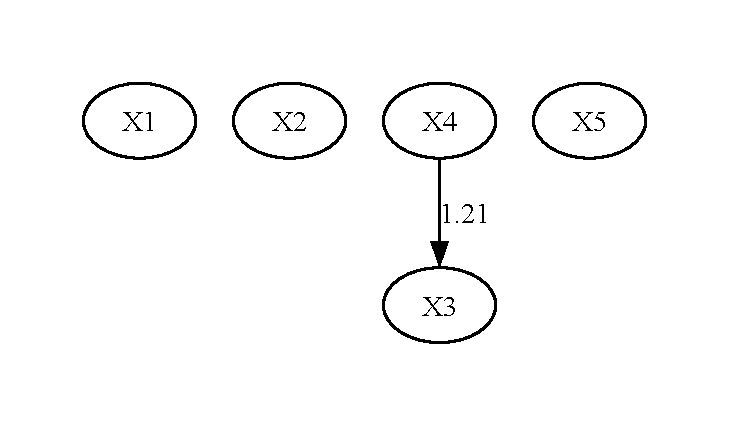
\includegraphics[height=0.3\textheight]{./demo_data/20241104_155654/Linear_Nongaussian_data/output_graph/initial_graph.pdf}
    \caption{Initial Graph}
\end{figure}

The above is the initial result graph produced by our algorithm.

The analysis indicates that X4 exerts a causal influence on X3, suggesting that changes or variations in X4 directly impact the state or behavior of X3. This relationship implies that fluctuations in the factors represented by X4 can lead to consequential effects on X3, potentially altering its dynamics or outcomes. Understanding this causal pathway is crucial, as it highlights the importance of considering how modifications in X4 can shape or inform the understanding of X3’s underlying mechanisms, thereby providing insights into the broader context in which these variables interact.

\subsection{Revised Graph}

\begin{minipage}[t]{0.6\linewidth}
    
        By using the method mentioned in Section 4.4, we provide a revised graph pruned with Bootstrap and LLM suggestion.
        Pruning results are as follows.
        
        Bootstrap doesn't force or forbid any edges.
            
        LLM doesn't force or forbid any edges.
            
        This structured approach ensures a comprehensive and methodical analysis of the causal relationships within the dataset.
        
\vfill
\end{minipage}
\hfill
\begin{minipage}[t]{0.4\linewidth}
    \begin{figure}[H]
        \centering
        \vspace{-0.5cm}
        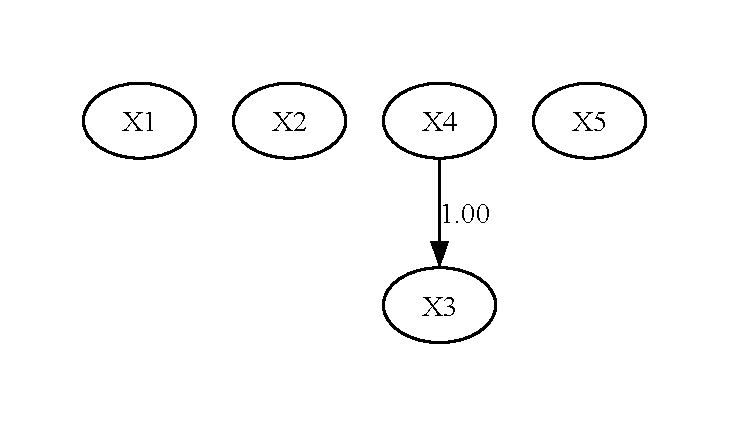
\includegraphics[width=\linewidth]{./demo_data/20241104_155654/Linear_Nongaussian_data/output_graph/revised_graph.pdf}
        \caption{\label{fig:corr}Revised Graph}
    \end{figure}
\end{minipage}


\subsection{Graph Reliability Analysis}

\begin{figure}[H]
    \centering
    \begin{subfigure}{0.49\textwidth}
        \centering
        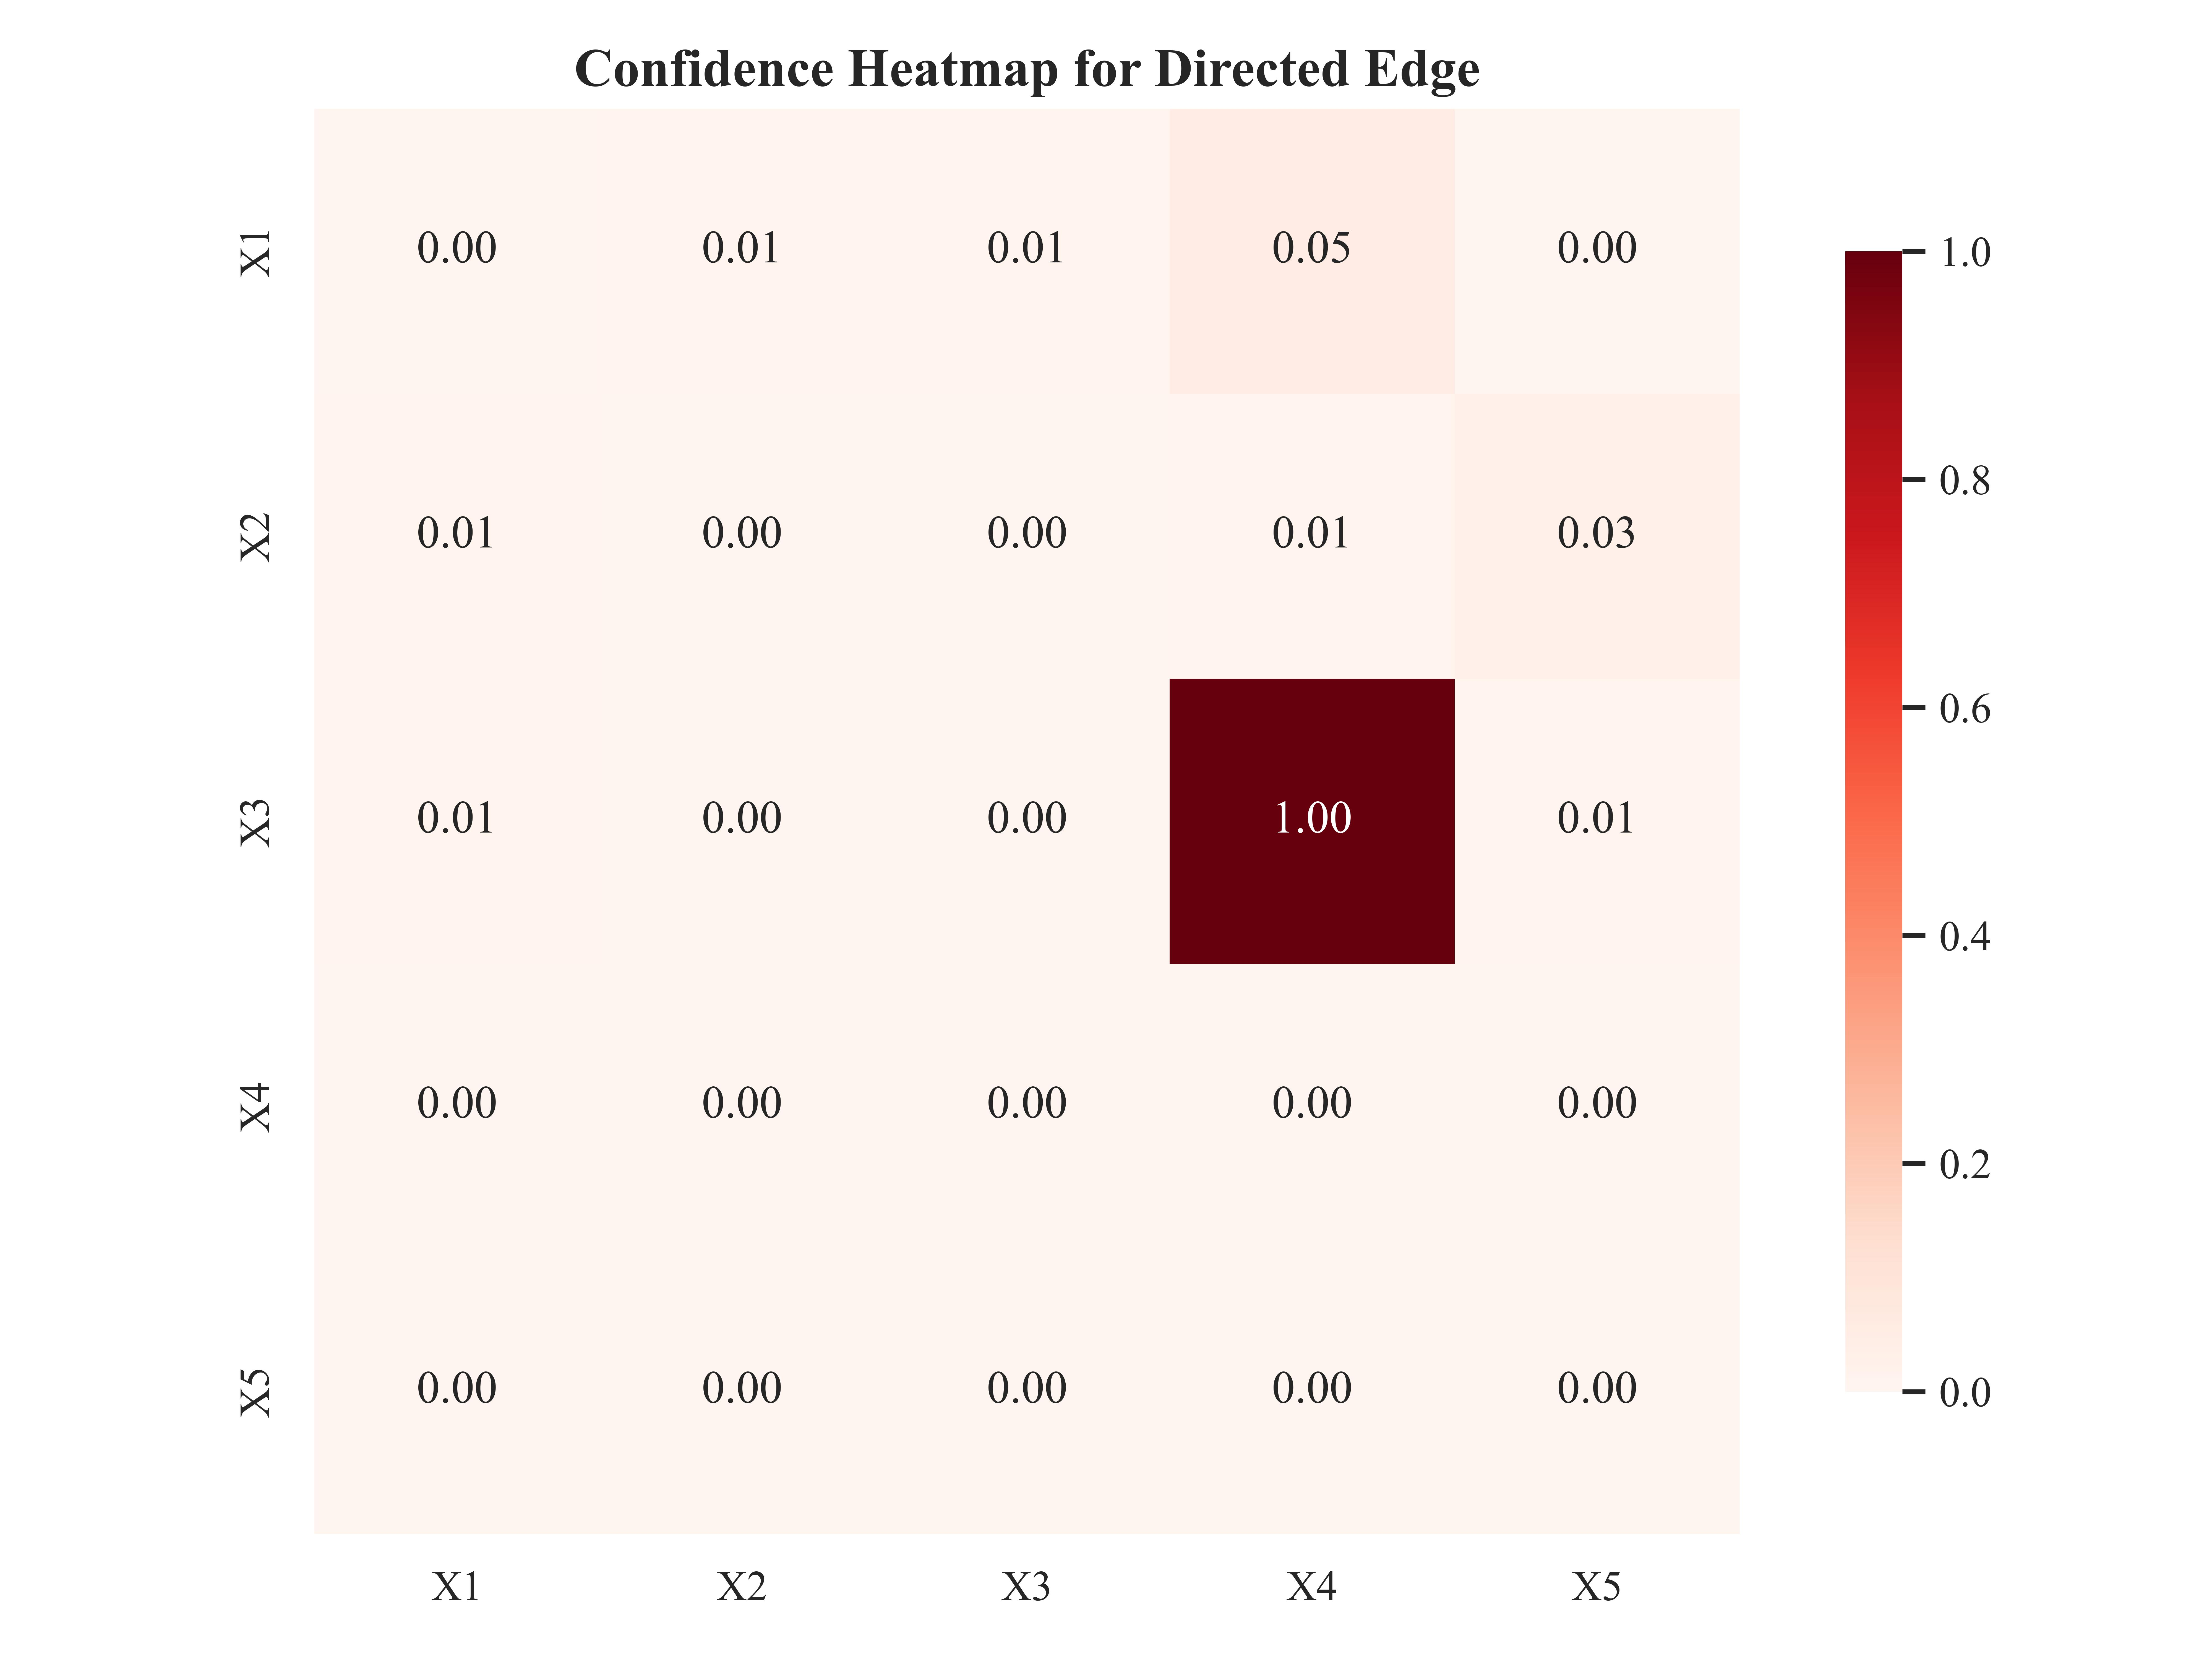
\includegraphics[width=\linewidth]{./demo_data/20241104_155654/Linear_Nongaussian_data/output_graph/certain_edges_confidence_heatmap.jpg}
        \caption{Directed Edge}
    \end{subfigure}
    \begin{subfigure}{0.49\textwidth}
        \centering
        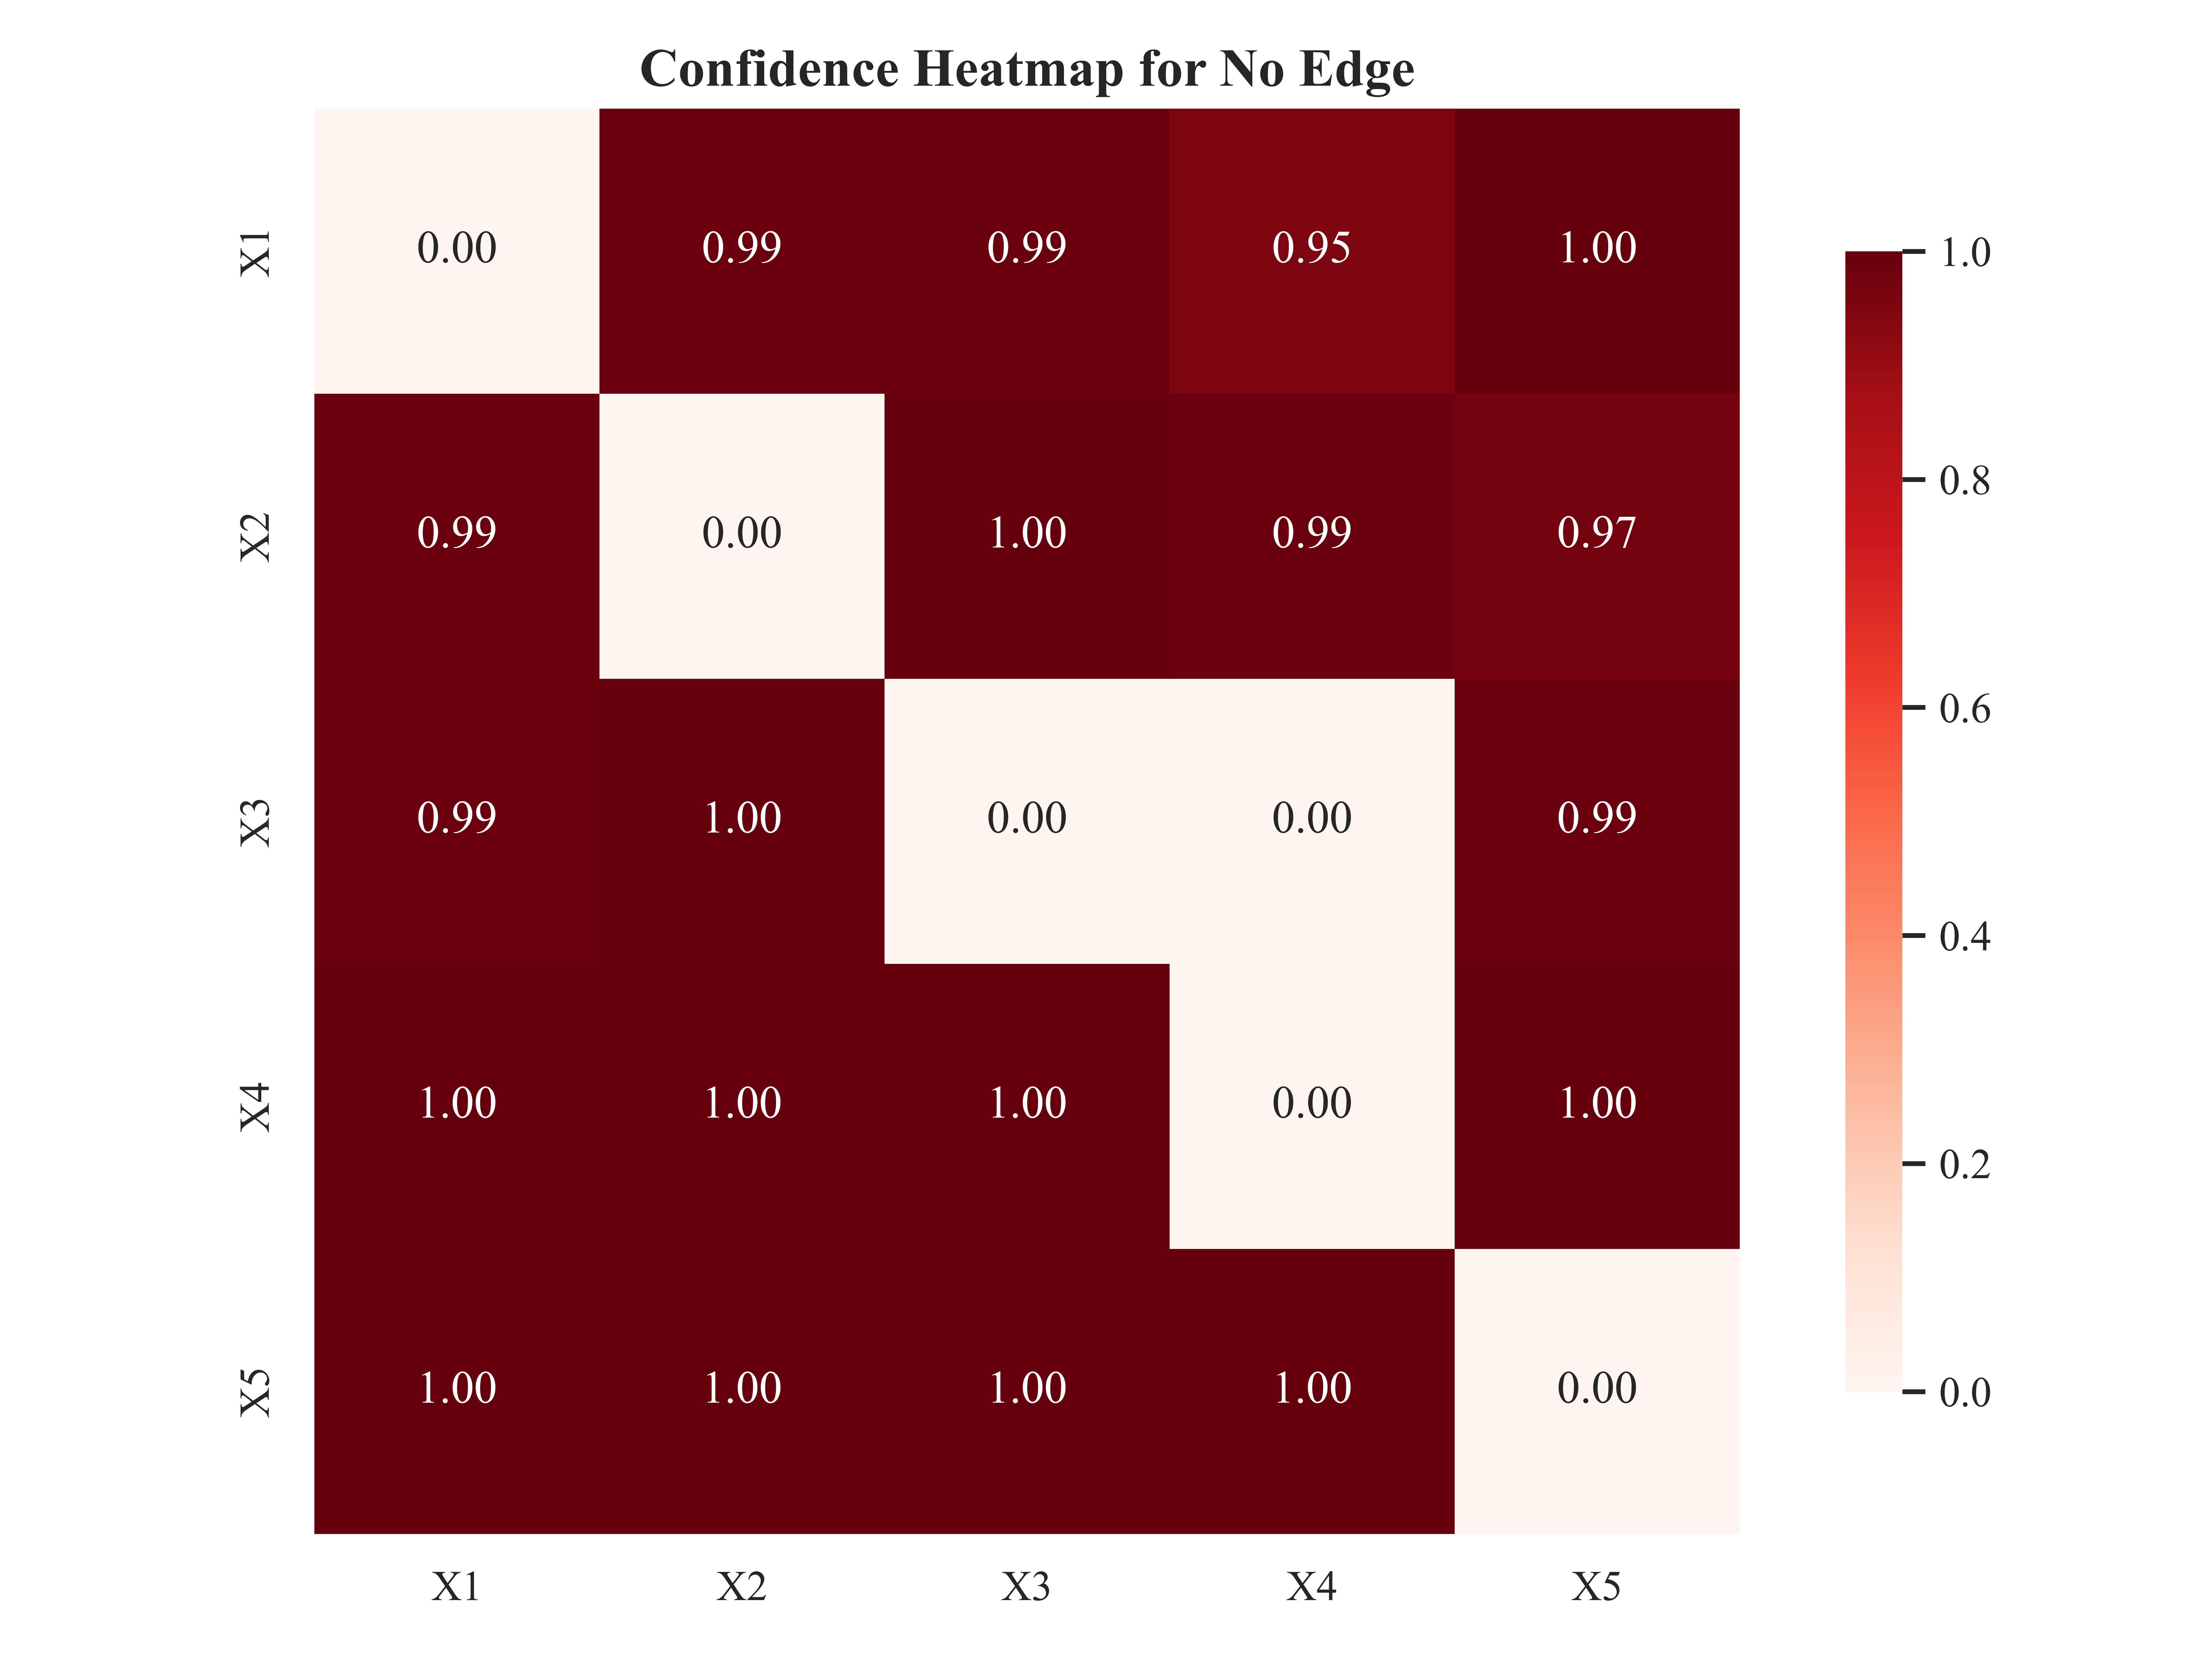
\includegraphics[width=\linewidth]{./demo_data/20241104_155654/Linear_Nongaussian_data/output_graph/non_existence_confidence_heatmap.jpg}
        \caption{No Edge}
    \end{subfigure}
    \caption{Confidence Heatmap of Different Edges}
\end{figure}        
The above heatmaps show the confidence probability we have on different kinds of edges, including directed edge ($\rightarrow$), No Edge, and probability of no edge. Based on the confidence probability heatmap and background knowledge, we can analyze the reliability of our graph.

From the statistics perspective, we have high confidence to believe that the edges with bootstrap probabilities close to 1 (not specified in your input but implied), represent strong causal relationships. However, we have no confidence in the edge X4 $\rightarrow$ X3, as indicated by a bootstrap probability of 0.0, suggesting that there is no support for this causal link based on the data. 

However, based on the expert knowledge, we know that there is no specific background knowledge to validate or invalidate any of the proposed relationships between these variables. This absence of context means we cannot substantiate any claims regarding the existence or non-existence of these edges with a high degree of certainty.

Therefore, the result of this causal graph is not reliable, especially given the complete lack of support for the edge X4 $\rightarrow$ X3 and the absence of any expert knowledge to affirm the other relationships with high confidence.

\end{document}